\documentclass[a4paper]{article}
\usepackage{geometry}
\usepackage{graphicx}
\usepackage{natbib}
\usepackage{amsmath}
\usepackage{amssymb}
\usepackage{amsthm}
\usepackage{paralist}
\usepackage{epstopdf}
\usepackage{tabularx}
\usepackage{longtable}
\usepackage{multirow}
\usepackage{multicol}
\usepackage[hidelinks]{hyperref}
\usepackage{fancyvrb}
\usepackage{algorithm}
\usepackage{algorithmic}
\usepackage{float}
\usepackage{paralist}
\usepackage[svgname]{xcolor}
\usepackage{enumerate}
\usepackage{array}
\usepackage{times}
\usepackage{tikz}
\usepackage{url}
\usepackage{fancyhdr}
\usepackage{comment}
\usepackage{environ}
\usepackage{times}
\usepackage{textcomp}
\usepackage{caption}


\urlstyle{rm}

\setlength\parindent{0pt} % Removes all indentation from paragraphs
\theoremstyle{definition}
\newtheorem{definition}{Definition}[]
\newtheorem{conjecture}{Conjecture}[]
\newtheorem{example}{Example}[]
\newtheorem{theorem}{Theorem}[]
\newtheorem{lemma}{Lemma}
\newtheorem{proposition}{Proposition}
\newtheorem{corollary}{Corollary}

\floatname{algorithm}{Procedure}
\renewcommand{\algorithmicrequire}{\textbf{Input:}}
\renewcommand{\algorithmicensure}{\textbf{Output:}}
\newcommand{\abs}[1]{\lvert#1\rvert}
\newcommand{\norm}[1]{\lVert#1\rVert}
\newcommand{\RR}{\mathbb{R}}
\newcommand{\CC}{\mathbb{C}}
\newcommand{\Nat}{\mathbb{N}}
\newcommand{\br}[1]{\{#1\}}
\DeclareMathOperator*{\argmin}{arg\,min}
\DeclareMathOperator*{\argmax}{arg\,max}
\renewcommand{\qedsymbol}{$\blacksquare$}

\definecolor{dkgreen}{rgb}{0,0.6,0}
\definecolor{gray}{rgb}{0.5,0.5,0.5}
\definecolor{mauve}{rgb}{0.58,0,0.82}

\newcommand{\Var}{\mathrm{Var}}
\newcommand{\Cov}{\mathrm{Cov}}

\newcommand{\vc}[1]{\boldsymbol{#1}}
\newcommand{\xv}{\vc{x}}
\newcommand{\Sigmav}{\vc{\Sigma}}
\newcommand{\alphav}{\vc{\alpha}}
\newcommand{\muv}{\vc{\mu}}

\newcommand{\red}[1]{\textcolor{red}{#1}}

\def\x{\mathbf x}
\def\y{\mathbf y}
\def\w{\mathbf w}
\def\v{\mathbf v}
\def\E{\mathbb E}
\def\V{\mathbb V}

% TO SHOW SOLUTIONS, include following (else comment out):
\newenvironment{soln}{
	\leavevmode\color{blue}\ignorespaces
}{}


\hypersetup{
	%    colorlinks,
	linkcolor={red!50!black},
	citecolor={blue!50!black},
	urlcolor={blue!80!black}
}

\geometry{
	top=1in,            % <-- you want to adjust this
	inner=1in,
	outer=1in,
	bottom=1in,
	headheight=3em,       % <-- and this
	headsep=2em,          % <-- and this
	footskip=3em,
}


\pagestyle{fancyplain}
\lhead{\fancyplain{}{Homework 1}}
\rhead{\fancyplain{}{CS 760 Machine Learning}}
\cfoot{\thepage}

\title{\textsc{Homework 1}} % Title

%%% NOTE:  Replace 'NAME HERE' etc., and delete any "\red{}" wrappers (so it won't show up as red)

\author{
	Daniel Szabo \\
	9074769625\\
} 

\date{}

\begin{document}
	
	\maketitle 
	
	
	\textbf{Instructions:} 
	This is a background self-test on the type of math we will encounter in class. If you find many questions intimidating, we suggest you drop 760 and take it again in the future when you are more prepared.
	
	Use this latex file as a template to develop your homework.
	Submit your homework on time as a single pdf file to Canvas.
	There is no need to submit the latex source or any code.
	Please check Piazza for updates about the homework.
	
	
	\section{Vectors and Matrices [6 pts]}
	Consider the matrix $X$ and the vectors $\mathbf{y}$ and $\textbf{z}$ below:
	$$
	X = \begin{pmatrix}
		3 & 2 \\ -7 & -5 \\
	\end{pmatrix}
	\qquad \mathbf{y} = \begin{pmatrix}
		2 \\ 1
	\end{pmatrix} \qquad \mathbf{z} = \begin{pmatrix}
		1 \\ -1
	\end{pmatrix}
	$$
	\begin{enumerate}
		\item 	Computer $\mathbf{y}^{T} X \mathbf{z}$\\
		\begin{soln} 
    	\begin{align*}
    		\mathbf{y}^{T} X \mathbf{z} = \mathbf{y}^T \begin{pmatrix}
    			1 \\ -2
    		\end{pmatrix} = 0
		\end{align*}
		     \end{soln}
		\item 	Is $X$ invertible? If so, give the inverse, and if no, explain why not.\\
        \begin{soln}
       	  The matrix $ X $ is invertible, and the inverse is 
       	  \[ X^{-1} = \begin{pmatrix}
       	  	5 & 2 \\ -7 & -3
       	  \end{pmatrix} \]
      	\end{soln}
	\end{enumerate}
	
	
	\section{Calculus [3 pts]}
	\begin{enumerate}
		\item If $y = e^{-x} + \arctan(z)x^{6/z} - \ln\cfrac{x}{x+1}$, what is the partial derivative of $y$ with respect to $x$?\\
		\begin{soln}  \begin{align*}
				\frac{\delta y}{\delta x} = -e^{-x} + \frac{6}{z}\arctan(z)x^{6/z-1} + \frac{x+1}{x} \frac{1}{x^2}
		\end{align*} \end{soln}
	\end{enumerate}
	
	
	
	
	\section{Probability and Statistics [10 pts]}
	Consider a sequence of data $S = (1, 1, 1, 0, 1)$ created by flipping a coin $x$ five times, where 0 denotes that the coin turned up heads and 1 denotes that it turned up tails.
	\begin{enumerate}
		\item 	(2.5 pts) What is the probability of observing this data, assuming it was generated by flipping a biased coin with $p(x=1) = 0.6$?
		
		\begin{soln}  
		Assuming the sequence is ordered, the probability would be $ .6^4\cdot .4 = .05184 $.
	\end{soln}
		
		\item 	(2.5 pts) Note that the probability of this data sample could be greater if the value of $p(x = 1)$ was not $0.6$, but instead some other value. What is the value that maximizes the probability of $S$? Please justify your answer.\\
		\begin{soln} We want to maximize the likelihood $ p^4(1-p) $, so taking the derivative we see this is equivalent to finding the root of $ 4p^3-5p^4 $ in $ (0,1] $. This root is at $ p=0.8 $, which is therefore the value that maximizes $ S $. This makes intuitive sense as well, as $ 0.8 $ of the flips were heads in the sample. \end{soln}
		
		\item 	(5 pts) Consider the following joint probability table where both $A$ and $B$ are binary random variables: 
		\begin{table}[htb]
			\centering
			\begin{tabular}{ccc}\hline
				A & B & $P(A, B)$  \\\hline
				0 & 0 & 0.3 \\
				0 & 1 & 0.1 \\
				1 & 0 & 0.1 \\
				1 & 1 & 0.5 \\\hline
			\end{tabular}
		\end{table}
		\begin{enumerate}
			\item 	What is $P(A = 0 | B = 1)$?\\
			 \begin{soln}  
			 \[ P(A = 0 | B = 1) = \frac{.1}{.1+.5} = \frac{1}{6} \]
		 	 \end{soln}
			 
			\item 	What is $P(A = 1 \vee B = 1 )$?\\
		     \begin{soln}  
		     	\[ P(A = 1 \vee B = 1 ) = .1+.1+.5 = .7 \]
		     \end{soln}
		\end{enumerate}
	\end{enumerate}
	
	
	\section{Big-O Notation [6 pts]}
	For each pair $(f, g)$ of functions below, list which of the following
	are true: $f(n) = O(g(n))$, $g(n) = O(f(n))$, both, or
	neither. Briefly justify your answers.
	\begin{enumerate}
		\item 	$f(n) = \ln(n)$, $g(n) = \log_{2}(n)$.\\
		\begin{soln}  
			Because $ \log_{2}(n) = \frac{\ln(n)}{\ln(e)} $, $ f(n) = \Theta(g(n))\implies f(n)=O(g(n)) $ and $ g(n) = O(f(n)) $
		\end{soln}
		
		\item 	$f(n) =  \log_{2}\log_{2}(n)$, $g(n) = \log_{2}(n)$.\\
		\begin{soln}  In this case, only $ f(n) = O(g(n)) $ because $ \lim\limits_{n\to\infty} \frac{f(n)}{g(n)} = 0 $. \end{soln}
		
		\item 	$f(n) = n!$, $g(n) = 2^n$.\\
		\begin{soln}  Here $ g(n) = O(f(n)) $ by Stirling's approximation, which says $ n!\sim \sqrt{n}\cdot n^n $ asymptotically, which is must faster than $ 2^n $. \end{soln}
	\end{enumerate}
	
	
	
	
	
	\section{Probability and Random Variables }
	\subsection{Probability [12.5 pts]}
	State true or false. Here $\Omega$ denotes the sample space and $A^c$ denotes the complement of the event $A$.
	\begin{enumerate}
		\item For any $A, B \subseteq \Omega$, $P(A|B)P(A) = P(B|A)P(B)$.\\
		\begin{soln} False. \\
			Multiplying both sides by $ P(B)P(A) $ gives that $ P(A)^3 = P(B)^3 $, which is not always true. \end{soln}
		
		\item For any $A, B \subseteq \Omega$, $P(A \cup B) = P(A) + P(B) - P(B \cap A)$.\\         
		\begin{soln}  True. \end{soln}
		
		\item For any $A, B, C \subseteq \Omega$ such that $P(B \cup C) > 0$,
		$\frac{P(A \cup B \cup C)}{P(B \cup C)} \geq P(A | B \cup C) P(B)$.\\ 
		\begin{soln}  True.\\
		This is equivalent to $ P(A\cup B \cup C) \geq P(A) P(B) $. WLOG say $ P(A)\geq P(B) $, which means $ P(A\cup B \cup C) \geq P(A) \geq P(A)P(B) $. \end{soln}
		
		\item For any $A, B\subseteq\Omega$ such that $P(B) > 0, P(A^c) > 0$,
		$P(B|A^C) + P(B|A) = 1$.\\ 
		\begin{soln}  True. \end{soln}
		
		\item If $A$ and $B$ are independent events, then $A^{c}$ and $B^{c}$ are independent.\\
		\begin{soln}  True.\\
		Applying De Morgan's law, $ P(A^cB^c) = 1-P(A\cup B) = 1-P(A)-P(B)+P(A)P(B) = 1-(1-P(A))P(B) - P(A) = P(A^c)-P(A^c)P(B) = P(A^c)P(B^c) $. \end{soln}
		
	\end{enumerate}
	
	\subsection{Discrete and Continuous Distributions [12.5 pts]}
	Match the distribution name to its probability density / mass
	function. Below, $|\xv| = k$.
	\begin{enumerate}[(a)]
		\begin{minipage}{0.3\linewidth}
			\item Gamma \begin{soln}  (j) \end{soln}
			\item Multinomial  \begin{soln}  (i) \end{soln}
			\item Laplace \begin{soln}  (h) \end{soln}
			\item Poisson \begin{soln} (l) \end{soln}
			\item Dirichlet  \begin{soln} (k) \end{soln}
			
		\end{minipage}
		\begin{minipage}{0.5\linewidth}
			\item $f(\xv; \Sigmav, \muv) = \frac{1}{\sqrt{(2\pi)^k \mathrm{det}(\Sigmav) }} \exp\left( -\frac{1}{2}
			(\xv - \muv)^T \Sigmav^{-1} (\xv - \muv)  \right)$
			\item $f(x; n, \alpha) = \binom{n}{x} \alpha^x (1 - \alpha)^{n-x}$
			for $x \in \{0,\ldots, n\}$; $0$ otherwise
			\item $f(x; b, \mu) = \frac{1}{2b} \exp\left( - \frac{|x - \mu|}{b} \right)$
			\item $f(\xv; n, \alphav) = \frac{n!}{\Pi_{i=1}^k x_i!}
			\Pi_{i=1}^k \alpha_i^{x_i}$ for $x_i \in \{0,\ldots,n\}$ and
			$\sum_{i=1}^k x_i = n$; $0$ otherwise
			\item $f(x; \alpha, \beta) = \frac{\beta^{\alpha}}{\Gamma(\alpha)} x^{\alpha -
				1}e^{-\beta x}$ for $x \in (0,+\infty)$; $0$ otherwise
			\item $f(\xv; \alphav) = \frac{\Gamma(\sum_{i=1}^k
				\alpha_i)}{\prod_{i=1}^k \Gamma(\alpha_i)} \prod_{i=1}^{k}
			x_i^{\alpha_i - 1}$ for $x_i \in (0,1)$ and $\sum_{i=1}^k x_i =
			1$; 0 otherwise
			\item $f(x; \lambda) = \lambda^x \frac{e^{-\lambda}}{x!}$ for all
			$x \in Z^+$; $0$ otherwise
		\end{minipage}
	\end{enumerate}
	
	\subsection{Mean and Variance [10 pts]}
	\begin{enumerate}
		\item Consider a random variable which follows a Binomial
		distribution: $X \sim \text{Binomial}(n, p)$.
		\begin{enumerate}
			\item What is the mean of the random variable?\\
			\begin{soln}  \[ \E[X]=np \] \end{soln}
			\item What is the variance of the random variable?\\
			\begin{soln}  \[ \Var(X) = np(1-p) \] \end{soln}
		\end{enumerate}
		
		\item Let $X$ be a random variable and
		$\mathbb{E}[X] = 1, \Var(X) = 1$. Compute the following values:
		\begin{enumerate}
			\item $\mathbb{E}[5X]$\\
			\begin{soln}  $ \E[5X]=5 $ by linearity of expectation. \end{soln}
			\item $\Var(5X)$\\
			\begin{soln}  $ \Var(5X)=5\Var(X) = 5 $. \end{soln}
			\item $\Var(X+5)$\\
			\begin{soln}  $ \Var(X+5)=\Var(X)=1 $. \end{soln}
		\end{enumerate}
	\end{enumerate}
	
	%\clearpage
	
	\subsection{Mutual and Conditional Independence [12 pts]}
	\begin{enumerate}
		\item (3 pts) If $X$ and $Y$ are independent random variables, show that
		$\mathbb{E}[XY] = \mathbb{E}[X]\mathbb{E}[Y]$.
		
		\begin{soln}  Expanding by the definition of expectation (assuming $ X,Y $ discrete for simplicity), we have  \begin{align*}
				\E[XY] &= \sum_{x,y\in\Omega} xy \Pr[X=x,Y=y] = \sum_{x,y\in\Omega} xy \Pr[X=x]\Pr[Y=y]\\ &=
				\sum_{x\in\Omega} x \Pr[X=x]\sum_{y\in\Omega} y \Pr[Y=y] = \E[X]\E[Y].
		\end{align*} The continuous case would be analogous with integrals replacing sums and density functions replacing probabilities. \end{soln}
		
		\item (3 pts) If $X$ and $Y$ are independent random variables, show that
		$\Var(X+Y) = \Var(X) + \Var(Y)$. \\
		Hint: $\Var(X+Y) = \Var(X) + 2\Cov(X, Y) + \Var(Y)$
		
		\begin{soln}  Directly applying the hint, $ \Var(X+Y) = \Var(X) + 2\Cov(X, Y) + \Var(Y) = \Var(X) + \Var(Y) $ because the convariance of two independent random variables is $ 0 $. \end{soln}
		
		\item (6 pts) If we roll two dice that behave independently of each
		other, will the result of the first die tell us something about the
		result of the second die? 
		
		\begin{soln}  It will not, because the two dice behave independently of each other. \end{soln}
		
		If, however, the first die's result is a 1,
		and someone tells you about a third event --- that the sum of the two
		results is even --- then given this information is the result of the second die
		independent of the first die? 
		
		\begin{soln}  It is no longer independent, the second die must be an odd number as well. The two dice are conditionally dependent on the third event. \end{soln}
	\end{enumerate}
	
	\subsection{Central Limit Theorem [3 pts]}
	Prove the following result.
	\begin{enumerate}
		\item Let $X_i\sim\mathcal{N}(0, 1)$ and $\bar{X} = \frac{1}{n}\sum_{i=1}^n X_i$, then the distribution of $\bar{X}$ satisfies 
		$$\sqrt{n}\bar{X}\overset{n\rightarrow\infty}{\longrightarrow}\mathcal{N}(0, 1)$$
		
		\begin{soln}  Look at the moment generating functions of $ \sqrt{n}\bar X $:
		\begin{align*}
			M_{\sqrt{n}\bar{X}}(t) = \E[e^{t\frac{1}{\sqrt{n}}\sum_{i=1}^n X_i}] = \E[e^{t\frac{1}{\sqrt{n}}X_1}]^n = M_{X_1}(t/\sqrt{n})^n.
	\end{align*} 
	Using the Taylor expansion of $ M_{X_1}(t/\sqrt{n}) $ about $ t=0 $, we see
	\begin{align*}
		M_{X_1}(t/\sqrt{n}) =& M_{X_1}(0) + M_{X_1}'(0) \frac{t}{\sqrt{n}} + M_{X_1}''(0) \frac{t^2}{2n} + o(t^2/n)\\
		=& 1 + \E[X_1]\frac{t}{\sqrt{n}} + \E[X_1^2]\frac{t^2}{2n} + o(t^2/n)\\
		=& 1+ \frac{t^2}{2n} + o(t^2/n).
	\end{align*}
	Looking at the limit of $ M_{\sqrt{n}\bar{X}}(t) $ as $ n\to \infty $, we see that the higher order terms vanish which means
	\[ \lim\limits_{n\to \infty} M_{\sqrt{n}\bar{X}}(t) = \lim\limits_{n\to \infty} (1+ \frac{t^2}{2n} + o(t^2/n))^n = \lim\limits_{n\to \infty} (1+ \frac{t^2}{2n})^n = e^{-\frac{t^2}{2}}. \]
	Now, using the fact that the MGF of the normal distribution is $ e^{-\frac{t^2}{2}} $, we see that the MGF of $ \sqrt{n}\bar{X} $ converges to that of $ \mathcal{N}(0,1) $, so the distribution converges as well. I used the proof in the wikipedia
	\color{red}\hyperref{https://en.wikipedia.org/wiki/Central_limit_theorem#Proof_of_classical_CLT}{}{}{page}\color{blue}~ for the CLT to help guide my proof.

\end{soln}
		
	\end{enumerate}
	
	
	
	\section{Linear algebra}
	
	
	\subsection{Norms [5 pts]}
	Draw the regions corresponding to vectors $\mathbf{x}\in\RR^2$ with the following norms:
	\begin{enumerate}
		\item 	$||\mathbf{x}||_1\leq 1$ (Recall that $||\mathbf{x}||_1 = \sum_i |x_i|$)

	\begin{soln}
		\begin{tikzpicture}
			\draw (-1.5,0) -- (1.5,0);
			\draw (0,-1.5) -- (0,1.5);
			\draw (-1,0) -- (0,-1) -- (1,0) -- (0,1) -- (-1,0);
		\end{tikzpicture}
	    % add figure filename, and remove % 
	    %    (this can be done by highlighting text and pressing "cmd + /" for sharelatex+mac)
	   % \begin{figure}[h!]
	   %     \centering
	   %     \includegraphics[width=0.4\textwidth]{FIGURE_FILENAME.pdf}  
	   %             % reference folder/figure.pdf here and adjust width
	   %     \captionsetup{labelformat=empty}
	   %     \caption{}
	   %     \label{fig:my_label}
	   % \end{figure}
	\end{soln}
		
		\item 	$||\mathbf{x}||_2 \leq 1$ (Recall that $||\mathbf{x}||_2 =\sqrt{\sum_i x_i^2}$)
			\begin{soln}
				
			\begin{tikzpicture}
				\draw (-1.5,0) -- (1.5,0);
				\draw (0,-1.5) -- (0,1.5);
				\draw (0,0) circle (1);
			\end{tikzpicture}
			% add figure filename, and remove % 
			%    (this can be done by highlighting text and pressing "cmd + /" for sharelatex+mac)
			% \begin{figure}[h!]
			%     \centering
			%     \includegraphics[width=0.4\textwidth]{FIGURE_FILENAME.pdf}  
			%             % reference folder/figure.pdf here and adjust width
			%     \captionsetup{labelformat=empty}
			%     \caption{}
			%     \label{fig:my_label}
			% \end{figure}
		\end{soln}
		\item 	$||\mathbf{x}||_\infty \leq 1$ (Recall that $||\mathbf{x}||_\infty = \max_i |x_i|$)
			\begin{soln}
				
			\begin{tikzpicture}
				\draw (-1.5,0) -- (1.5,0);
				\draw (0,-1.5) -- (0,1.5);
				\draw (-1,-1) rectangle (1,1);
			\end{tikzpicture}
			% add figure filename, and remove % 
			%    (this can be done by highlighting text and pressing "cmd + /" for sharelatex+mac)
			% \begin{figure}[h!]
			%     \centering
			%     \includegraphics[width=0.4\textwidth]{FIGURE_FILENAME.pdf}  
			%             % reference folder/figure.pdf here and adjust width
			%     \captionsetup{labelformat=empty}
			%     \caption{}
			%     \label{fig:my_label}
			% \end{figure}
		\end{soln}
	\end{enumerate}
	
	For $M = \begin{pmatrix}
		5 & 0 & 0 \\ 0 & 7 & 0 \\ 0 & 0 & 3
		
	\end{pmatrix}$, Calculate the following norms.
	\begin{enumerate}\addtocounter{enumi}{3}
		\item $||M||_{2}$ (L2 norm) \\
		\begin{soln}  The L2 norm is just the maximum eigenvalue, so $ ||M||_{2} = 7 $. \end{soln}
		
		\item $||M||_{F}$ (Frobenius norm)\\
		\begin{soln}  $ ||M||_{F} = \sqrt{83} = 9.1104335791443 $. \end{soln}
		
		
	\end{enumerate}
	
	
	
	\subsection{Geometry [10 pts]}
	Prove the following.  Provide all steps.
	\begin{enumerate}
		\item 	The smallest Euclidean distance from the origin to some point $\mathbf{x}$ in the hyperplane $\mathbf{w}^{T}\mathbf{x} + b = 0$ is $\frac{|b|}{||\mathbf{w}||_2}$.  You may assume $\mathbf{w} \neq 0$.\\
		\begin{soln}  Say the distance was $ \frac{|b|}{||\mathbf{w}||_2} - \varepsilon $ for some $ \varepsilon>0 $. Then there is some unit vector $ \mathbf{u} $ such that 
		\begin{align*}
			&\mathbf{w}^{T} (\frac{|b|}{||\mathbf{w}||_2} - \varepsilon) \mathbf{u} + b \\
			=& \mathbf{w}^{T} \frac{|b|}{||\mathbf{w}||_2} \mathbf{u} + b - \varepsilon\mathbf{w}^T\mathbf{u}\\
			\leq& \mathbf{w}^{T} \frac{|b|}{||\mathbf{w}||_2} \frac{ \mathbf{w}}{\| \mathbf{w} \|_2} + b - \varepsilon\mathbf{w}^T\frac{\mathbf{w}}{\| \mathbf{w} \|_2}\\
			=& |b| + b - \varepsilon \|\mathbf{w}\|_2\\
			<& 0 \quad \text{If } b\leq0.
		\end{align*}
		If $ b>0 $, we can repeat the same argument with $ \mathbf{u}=-\frac{\mathbf{w}}{\| \mathbf{w} \|_2} $ to show $ \mathbf{w}^{T}\mathbf{x} + b $ is bounded below by $ 0 $.
		\end{soln}
		
		\item 	The Euclidean distance between two parallel hyperplane $\mathbf{w}^{T}\mathbf{x} + b_1 = 0$ and $\mathbf{w}^{T}\mathbf{x} + b_2 = 0$ is $\frac{|b_1 - b_2|}{||\mathbf{w}||_2}$ (Hint: you can use the result from the last question to help you prove this one).
		
		\begin{soln}  We can simply transform both planes by $ b_2 $ so that the origin lines on the second plane. We saw in problem $ 1. $ that the shortest distance from $ \mathbf{w}^{T}\mathbf{x} + b_1 - b_2 = 0 $ to the origin is $ \frac{|b_1 - b_2|}{||\mathbf{w}||_2} $, and because these planes are parallel, that is the shortest distance at any point.
		\end{soln}
		
	\end{enumerate}
	
	
	
	\section{Programming Skills [10 pts]}
	Sampling from a distribution.  For each question, submit a scatter plot (you will have 2 plots in total).  Make sure the axes for all plots have the same ranges.
	\begin{enumerate}
		\item Make a scatter plot by drawing 100 items from a two dimensional Gaussian $N((1, -1)^{T}, 2I)$, where I is an identity matrix in $\mathbb{R}^{2 \times 2}$.
		
			\begin{soln}
			
			% add figure filename, and remove % 
			%    (this can be done by highlighting text and pressing "cmd + /" for sharelatex+mac)
			 \begin{figure}[h!]
			     \centering
			     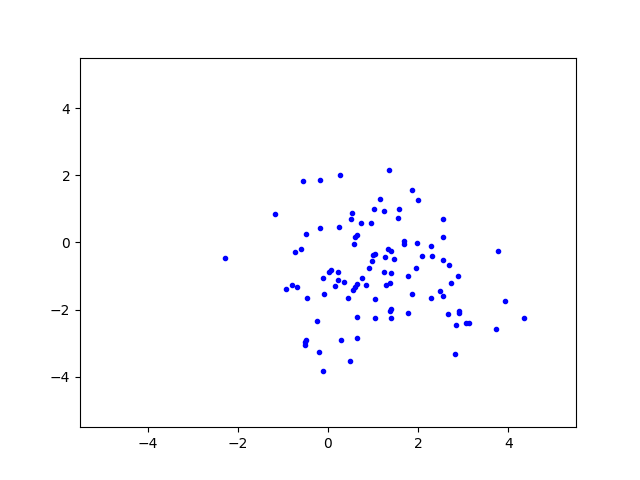
\includegraphics[width=0.4\textwidth]{firstscatter.png}  
			             % reference folder/figure.pdf here and adjust width
			     \captionsetup{labelformat=empty}
			     \caption{}
			     \label{fig:fig1}
			 \end{figure}
		\end{soln}
	
		\item Make a scatter plot by drawing 100 items from a mixture distribution 
		$0.3 N\left((5, 0)^{T}, \begin{pmatrix} 1 & 0.25 \\ 0.25 & 1\\ \end{pmatrix}\right)
		+0.7 N\left((-5, 0)^{T}, \begin{pmatrix} 1 & -0.25 \\ -0.25 & 1\\ \end{pmatrix}\right)
		$.
		
		\begin{soln}
			
		% add figure filename, and remove % 
		%    (this can be done by highlighting text and pressing "cmd + /" for sharelatex+mac)
		 \begin{figure}[h!]
		     \centering
		     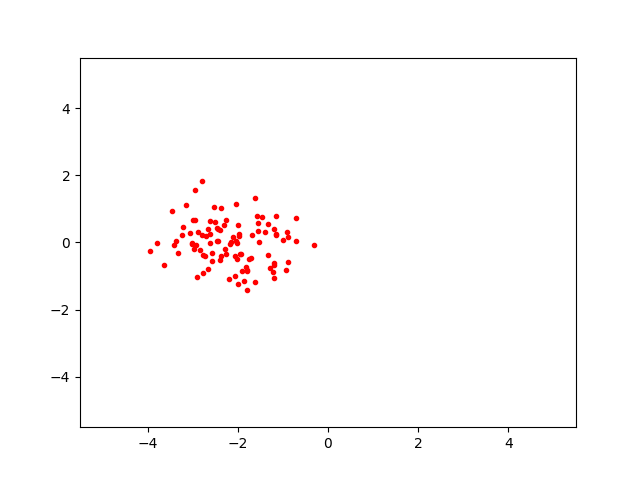
\includegraphics[width=0.4\textwidth]{secondscatter.png}  
		             % reference folder/figure.pdf here and adjust width
		     \captionsetup{labelformat=empty}
		     \caption{}
		     \label{fig:fig2}
		 \end{figure}
	\end{soln}
	\end{enumerate}
	
	
	\bibliographystyle{apalike}
	
	
	%----------------------------------------------------------------------------------------
	
	
\end{document}
